\definecolor{B128first}{HTML}{F6C928}
\definecolor{B256}{HTML}{36827F}
\definecolor{B128second}{HTML}{96A654}
\definecolor{B1024}{HTML}{464D77}

\begin{figure*}[t]
    \centering
    % \vspace{-0.6cm}
    %
    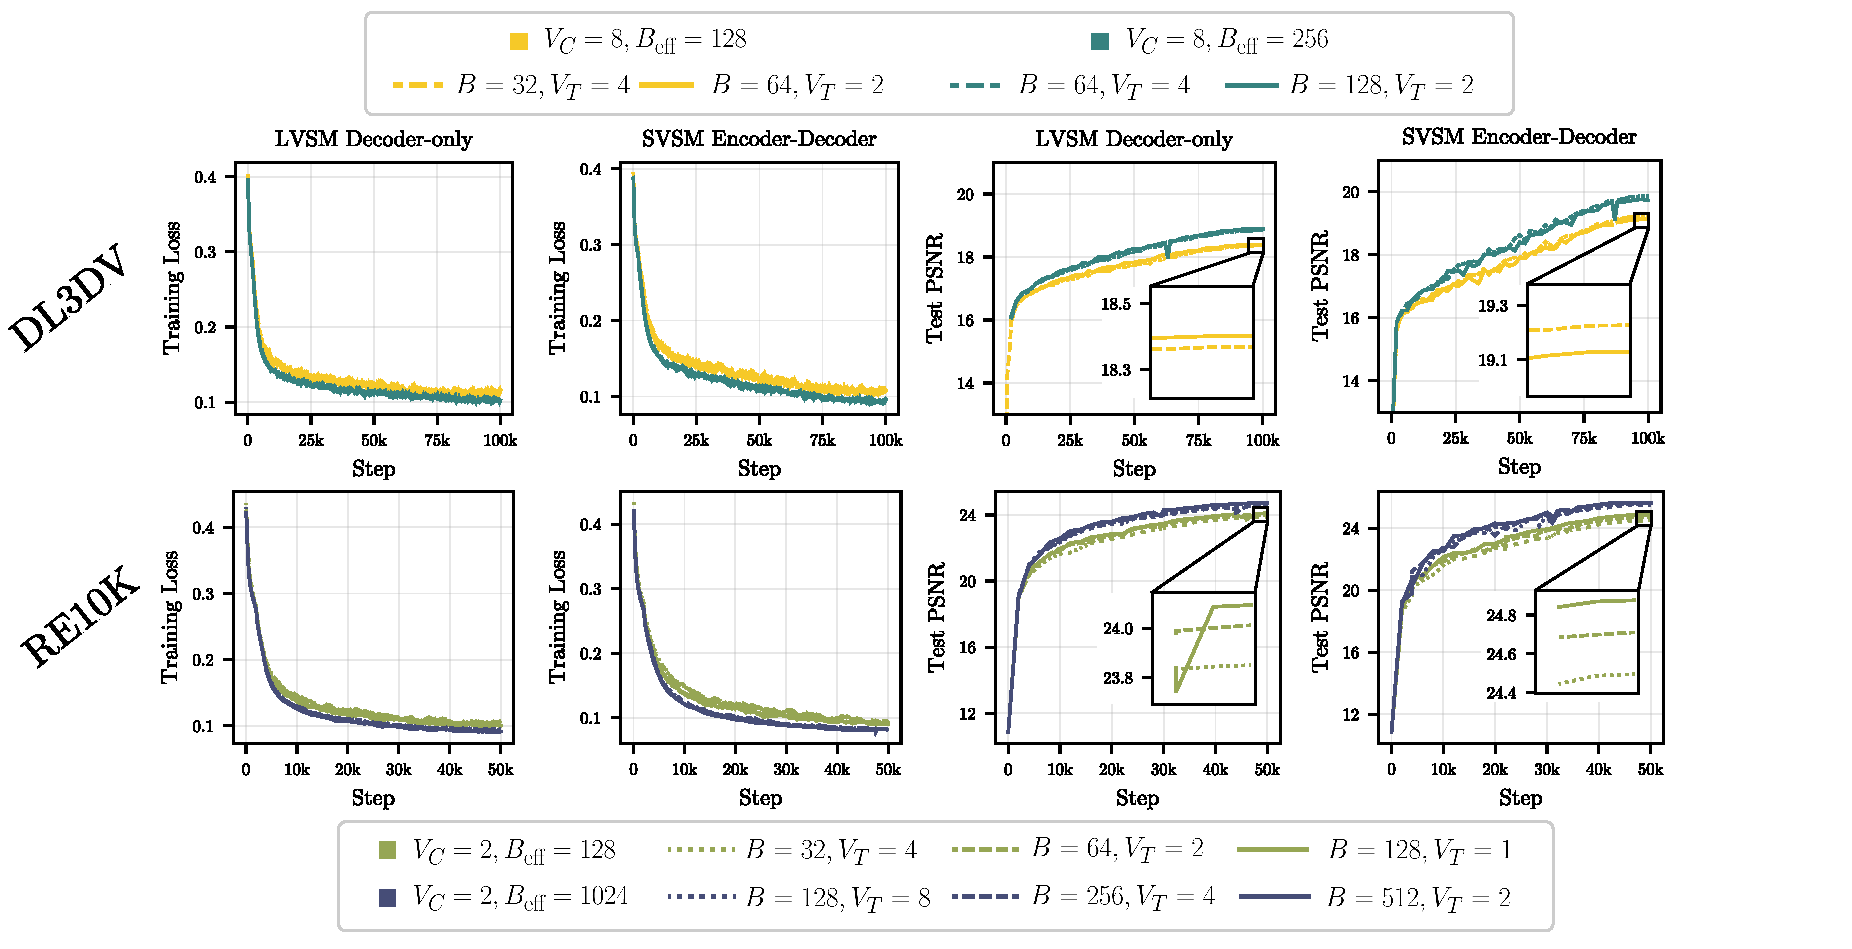
\includegraphics[width=\textwidth]{images/effective_batch_all.pdf}
    %
    \vspace{-0.8cm}
    \caption{\textbf{Effective Batch Size}. Training loss (smoothed with a rolling-average) and test PSNR measured throughout training across various paired $B$ and $V_T$ runs provide evidence for our effective batch size hypothesis: Models trained with the same product of number of scenes in the batch $B$ and number of reconstruction target views $V_T$, \emph{i.e.} runs with the same \emph{effective batch size} $B_{\text{eff}}$, perform the same and are colored identically. On $V_C = 8$ \textbf{(top)}, we sweep across $B_{\text{eff}} = $ \textcolor{B128first}{128}, \textcolor{B256}{256} on DL3DV, and on $V_C = 2$ \textbf{(bottom)}, we sweep across $B_{\text{eff}} =$ \textcolor{B128second}{128}, \textcolor{B1024}{1024} on RealEstate10K.
    \vspace{-1\baselineskip}
} % Main caption
    \label{fig:effective-batch} % Main label
\end{figure*}
\section{Encoder-Decoder View Synthesis}
\label{sec:architecture}
% As discussed in \secref{sec:background-scale}, 
% the decoder-only LVSM model must recompute scene information from the context views each time it renders a new target view. While it allows the model to focus only on information in the context views that is relevant to the given rendering target, it also prevents the model from leveraging a re-usable scene representation to reduce the cost of rendering multiple targets with the same context.
% % the decoder-only LVSM model processes scene information directly from the raw pixels every time it renders a new target view. This design prevents the model from leveraging shared scene encoding to save the cost of rendering.
% % As a result, shared information across multiple views cannot be preprocessed in an amortized manner and instead must be recomputed each time a new target image is rendered, making both the training and inference largely inefficient.
% The encoder-decoder variant of LVSM also suffers a similar drawback due to bidirectionality as the renderer must also update the scene tokens in conjunction with those of the target, leading to large self-attention maps. Due to these inefficiencies, it is costly to scale either LVSM variant with additional context or target views. 

As discussed in \secref{sec:intro} and \secref{sec:background-scale}, the decoder-only LVSM may not be the most compute-optimal due to the recomputation per-target view rendered. 
This motivates us to seek an alternative model with a fixed scene representation that can be decoded in a purely \emph{unidirectional} manner (\emph{i.e.} via cross attention) to reduce the cost of rendering and avoid redundant reprocessing of context information. To this extent, we introduce the Scalable View Synthesis Model (SVSM), which can be viewed as a simple modification to encoder-decoder LVSM.
%
Specifically, our architecture implements \eqref{eq:view_synthesis} by first processing the context set $\mathfrak{C}$ with a transformer encoder, producing a set of latent tokens (a ``scene representation'') $\mathbf{z} = \mathcal E[\mathfrak{C}]$.
The encoder $\mathcal E$ is standard transformer with full bidirectional self-attention.
Unlike encoder-decoder LVSM, we do not employ a fixed-size scene representation, but instead take the set of encoded context image patch tokens as the scene representation to avoid introducing a bottleneck. To render a novel view, a cross-attention based decoder $\mathcal D$ ingests the target configuration and the fixed scene latent tokens $\mathbf{z}$ to render the target view, $\tilde{I} = D \big[\mathbf{z}, \, \tpose, \tK \big]$. 
%
To render multiple images of the same scene, we only require encoding the context set once, re-using the scene embedding $\mathbf{z}$. As with LVSM, each novel view is decoded independently given $\mathbf{z}$ (i.e., there is no interaction between target views). However, because the decoder uses cross-attention rather than bidirectional self-attention over all tokens, these independent target views can be decoded in parallel, without redundant recomputation of the scene representation.
% Thus, rendering multiple target views using the same context images requires encoding the scene representation \emph{once}, and repeatedly calling \emph{only} the efficient unidirectional renderer.  

% where a target view is rendered via cross-attention with a latent scene representation (\figref{fig:lvsm-svsm}, right).
% This enables the model to proactively discard information irrelevant to the target view and focus its resource to target-specific parts. However, 
% We introduce an alternative encoder-decoder architecture to tackle the generalizable novel view synthesis problem, which we coin the Scalable View Synthesis Model (SVSM). In the experiments section, we will demonstrate that this architecture is dramatically more FLOP-efficient than the decoder-only LVSM architecture.
%
% We contrast our architecture with the SOTA LVSM decoder-only model in \figref{fig:lvsm-svsm}. There are two differences of note: 1) the presence of an encoder, and 2) the cross-attention based decoder. 
%
% Our architecture implements \eqref{eq:view_synthesis} by first processing the context set $\mathcal{C}$ with a transformer encoder, producing a set of latent tokens (a ``scene representation'') $\mathbf{z} = E(\mathcal{C})$. To encode the context set, we leverage a standard transformer with full bidirectional attention.
% %
% To render a novel view, a cross-attention based decoder or renderer $D$ ingests the target pose as well as the set of latent tokens $\mathbf{z}$ to map them to a target view, $\hat{I} = D \big[\mathbf{z}, \, \tpose, \tK \big]$.

% To render multiple images of the same scene, we only require encoding the context set \emph{once}, re-using the scene embedding $\mathbf{z}$. The cross-attention based decoder then enables parallel decoding of a flexible number of target views.
% %
% In other words, assuming most of the compute is due to the MLP layers (\textbf{see Supp.}), rendering $V_T$ target views requires
% $\mathcal O(V_C + V_T)$
% FLOPs. 
% %
% In the limit where we are rendering many more target views than context views which is the major practical use case, this simplifies to $\mathcal O(V_T)$. This reduction of compute is exactly where the advantage of SVSM lies.
To be more concrete, this architecture reduces the complexity of rendering $V_T$ targets to
\begin{equation}\label{eqn:svsm-flops}
\begin{split}
    \computeMLP^{\text{(SVSM)}} & \propto V_T + V_C
    \\
    \computeAttn^{\text{(SVSM)}} & \propto V_C\times (V_T + V_C).
\end{split}
\end{equation}
%
In other words, assuming most of the compute is due to the MLP layers (see \suppref{supp:flop-calcs}), rendering $V_T$ target views requires $\mathcal O(V_T + V_C)$ FLOPs. In the limit of inference where $V_T \gg V_C$, this reduces to $\mathcal O(V_T)$, in stark contrast to the $\mathcal O(V_TV_C + V_T)$ of LVSM (see \eqref{eqn:lvsm-flops}). Further, the benefit of this paradigm extends beyond inference. As long as we are training with multiple target views, as is standard practice~\citep{charatan2024pixelsplat, jin2024lvsm, sajjadi2022scene, zhang2024gs}, the parallel nature of unidirectional decoding can save substantial training compute.
% can also save a substantial amount of compute during training.


% FLOPs. 
% %
% In the limit where $V_T{>>}V_C$, which is the major practical use case, this simplifies to $\mathcal O(V_T)$. This reduction of compute is exactly where the advantage of SVSM lies.

However, this reduction comes with a cost. Unlike LVSM, our encoder cannot proactively discard information irrelevant to the target view but instead needs to encode all necessary information for rendering \emph{any} target view. Indeed, parameter count and training steps being equal, SVSM performs worse than LVSM. However, as we will show, SVMS’s amortized rendering enables us to dramatically increase its size and training steps, such that when normalized by compute budget, SVSM significantly outperforms LVSM.

% This can be viewed as a source inefficiency, so the compute-optimality of our model hinges on how well we amortize the cost of this scene representation thorough repeated rendering, assuming the latter can provide a significant benefit as a training objective. 
% To this point, our proposed unidirectional model cannot directly compete with an LVSM model of the same size. 
% Indeed, our unidirectional model cannot directly compete with an LVSM model of the same size. However, as we will show, SVSM can be made more efficient by leveraging its superior scalability with a larger number of target $V_T$ views,  enabling us to increase the parameter count by a significant factor compared to LVSM. In the following sections, we empirically confirm that the advantages of a unidirectional model substantially outweigh those of a bidirectional model,  both for training and inference.




% In this section, we recap the LVSM architecture and introduce our encoder-decoder architecture,  Both are pictured in Fig. \ref{fig:lvsm-svsm}. In summary, we simplify the encoder structure and make the decoder lightweight. 

\section{The Effective Batch Size for View Synthesis}
\label{sec:effective-batch}

% The implicit standard practice employed by prior work~\citep{charatan2024pixelsplat, jin2024lvsm, sajjadi2022scene, zhang2024gs} has been to reconstruct multiple different target views from a single scene during training. However, the consequences of this approach have never been fully analyzed. To this point, we propose and empirically validate the \emph{effective batch hypothesis}, which argues that reconstructing multiple target views per scene effectively multiplies the batch size.
As the cost of a forward pass scales both with the number of different scenes (the batch size $B$) as well as the number of target views ($V_T$) that we seek to render per scene, this introduces an additional hyperparameter into the training regime: What is the \emph{optimal} trade-off between the number of target views and the number of different scenes? 
We study this question empirically and reveal that what matters is the \emph{product} of target views and batch size, which we call the \emph{effective batch size} of a NVS model. 
% To better understand this impact of using multiple different target views for training, we propose the concept of ``effective batch size'' in novel view synthesis. 
\vspace{-1\baselineskip}



\paragraph{Analysis Setup.}
%
We define effective bath size as $B_{\text{eff}} \equiv B \cdot V_T$, where $B$ is the number of scenes in a training batch, and $V_T$ is the number of rendering targets used per training scene.
%
We train both decoder-only LVSM and the proposed SVSM models across two datasets --- DL3DV~\cite{ling2024dl3dv} and RealEstate10K~\cite{zhou2018stereo} (RE10K) --- with $V_C = 8$ and $V_C = 2$ while holding $B_{\text{eff}}$ constant and varying $B$ and $V_T$. Specifically, we test $B_{\text{eff}} = 128$ on both datasets, and additionally test $B_{\text{eff}} = 1024$ on RE10K and $B_{\text{eff}} = 256$ on DL3DV. For DL3DV we use the official test-train split, and for RE10K, we use the pixelSplat~\citep{charatan2024pixelsplat} test-train split.
%
Further training details are outlined in \suppref{supp:exp-details}.
% Further, we track the test metrics and train loss throughout training time to see whether the training dynamics are indeed similar across runs of the same effective batch, which should occur if additional target views play a similar role in reducing gradient noise, as batch size does.

% to see whether the curves align, indicating an ``effective batch size'' effect.
% \vspace{-1\baselineskip}



\paragraph{Effective Batch Size is What Matters.} Results for all training runs are shown in \figref{fig:effective-batch}. Remarkably, in all cases -- across both models, both $V_C$ settings, and all $B_{\text{eff}}$ sets -- the test metric and the training loss behavior remain approximately constant along a $B_{\text{eff}}$-level set. This effect is especially clear in the $V_C = 8$ case, where the test PSNR varies by at most $\pm 0.1$ and remains present in the $V_C = 2$ case, where the variation is at most $\pm 0.2$~PSNR. Tuning $B$ and $V_T$ within the same effective batch size $B_{\text{eff}}$ does not result in significant difference in the final performance outcome, we exclude this degree of freedom from our subsequent analyses and treat $B_{\text{eff}}$ as the true batch size. 

% We hypothesize that the stronger consistency observed for $V_C = 8$ arises from the wider baselines inherent in that training configuration -- each additional view provides a learning signal as rich as adding a new scene -- though we leave a more rigorous investigation of this effect to future work.

%Following \citet{tuningplaybookgithub}, we do not tune over the (effective) batch size for model performance. Instead, we use the training FLOPS as the invariant measure to assess the compute-optimality.  
% \vspace{-1\baselineskip}

% \todo{rework transition between these two sections or potentially merge them as they are a little repetitive}


\paragraph{SVSM Enables Compute-Optimal Tradeoff.}
%
How can we interpret this result through the lens of compute-optimiality? For the LVSM decoder-only model, the training compute scales as 
\begin{equation}
    \compute{}^{\text{(LVSM)}} \propto B V_T (V_C + 1) = B_{\text{eff}}(V_C + 1).
\end{equation}
Thus, any training settings within constant $B_{\text{eff}}$ not only achieve within-noise results (as per our effective batch result), but also require the same number of FLOPs. This means for the decoder-only model there is \emph{no advantage to be gained by tuning $V_T$}. In contrast, for the SVSM model, training compute is proportional to
\begin{equation}
    \compute{}^{\text{(SVSM)}} \propto B(V_C + V_T) = B_{\text{eff}} + BV_C.
\end{equation}
Therefore, by reducing $B$ and increasing $V_T$, one can achieve the same effective batch size -- and consequently, the same performance -- with lower compute cost. This justifies our original motivation for a model design that efficiently decodes multiple $V_T$.


% \textbf{SVSM has a better pareto frontier.} 

% %
% \begin{itemize}
%     \item Why do we have better frontier? Reference flop calculations
%     \item Why is this justified? effective batch size sweep proof
%     \item maybe some comments about how this gives understanding for what all this multiple view training has been
%     \item currently have some: straggles of RE10k 2 view, good DL3DV 8 view. maybe should add DL3DV 4 view.
% \end{itemize}
%


%
% As discussed in sec. \ref{sec:architecture}, a major advantage of the SVSM architecture is the ability to compute multiple target views within a given scene. This is immediately helpful at inference time where multiple target poses can be decoded in parallel. 




